%%%%%%%%%%%%%%%%%%%%%%%%%%%%%%%%%%%%%%%%%
% Memo
% LaTeX Template
% Version 1.0 (30/12/13)
%
% This template has been downloaded from:
% http://www.LaTeXTemplates.com
%
% Original author:
% Rob Oakes (http://www.oak-tree.us) with modifications by:
% Vel (vel@latextemplates.com)
%
% License:
% CC BY-NC-SA 3.0 (http://creativecommons.org/licenses/by-nc-sa/3.0/)
%
%%%%%%%%%%%%%%%%%%%%%%%%%%%%%%%%%%%%%%%%%

\documentclass[letterpaper,11pt]{texMemo} % Set the paper size (letterpaper, a4paper, etc) and font size (10pt, 11pt or 12pt)

\usepackage{parskip} % Adds spacing between paragraphs
\setlength{\parindent}{15pt} % Indent paragraphs

%----------------------------------------------------------------------------------------
%	MEMO INFORMATION
%----------------------------------------------------------------------------------------

%\memoto{Mr. Lynch } % Recipient(s)

%\memofrom{Mike Patel} % Sender(s)

\memosubject{Syed Raza Haider} % Memo subject

\memodate{\today} % Date, set to \today for automatically printing todays date

%\logo{
\includegraphics[width=0.3\textwidth]{logo.png}} % Institution logo at the top right of the memo, comment out this line for no logo

%----------------------------------------------------------------------------------------

\begin{document}

\maketitle % Print the memo header information

%----------------------------------------------------------------------------------------
%	MEMO CONTENT
%----------------------------------------------------------------------------------------
\section{Persona Development}

John is a 38-year-old project manager at a tech company, where he plays a crucial role in the company's success by leading multiple projects. His demanding lifestyle includes long work hours and frequent business travel, making it difficult for him to balance his work commitments with staying fit. Although John was very active during his university years, participating in running groups, his fitness routine has suffered over the years.

John wants to regain control of his health, focusing on losing weight and improving his stamina without compromising his work-life balance. He is looking for a personalized fitness plan that accommodates both indoor and outdoor activities and fits into his hectic schedule. Additionally, he appreciates reminders to stand up and stay active during long periods of sitting.

As a tech-savvy individual, John is comfortable using apps and expects intuitive interfaces with seamless integration to his wearable devices and social platforms.


\section{Contexts of use}

\begin{enumerate}
	
	\item \bf{Daily Workout:}
	\normalfont{Recommend users daily exercise tailored to their activity level and previous data. }
	
	\item  \bfseries{Calorie and Nutrition Logging:}
	\normalfont{Allow users to add calories intake of their meals and adjust their goals accordingly}
	
	\item  \bf{Sharing pictures and fitness:}  \normalfont{Allow users to share their workout summaries and achievements with friends and family via social media for encouragement.}


\subsection{Context 2: During Business Travel  }
Because John's job involves frequent business trips, maintaining a consistent fitness routine is challenging. ActivePro steps in by offering personalized training tips and suggesting available resources based on his current location, such as nearby parks for running or outdoor gyms. Additionally, the app helps him track his nutrition by recommending healthy restaurants and meal options, ensuring he stays on top of his fitness goals even while traveling.

\section{Scenario: Morning Workout}

John wakes up at 6:00 a.m. after a solid 8 hours of sleep. His schedule is packed for the day, but he starts by opening ActivePro, which greets him with a welcome message and a personalized workout plan, taking into account his busy day ahead. Since he completed a high-intensity workout the day before, ActivePro recommends a 20-minute low-impact bodyweight session. John follows the suggested routine, which includes stretching, 20 push-ups, and breathing exercises.

After completing the workout, ActivePro congratulates him for staying consistent and reminds him to log his breakfast. He quickly inputs his meal into the app, which then adjusts his daily calorie goals accordingly. Before heading to work, John shares his workout summary on social media, where his friends and family cheer him on, boosting his motivation and setting a positive tone for the rest of his day.

\section{Mini Use Case: Flowchart for Core Task (Workout Selection and Execution}

For this mini use case, the task would be to select and execute a daily workout using ActivePro as demonstrated in a flow chart:


\begin{figure}[h]
	\centering
	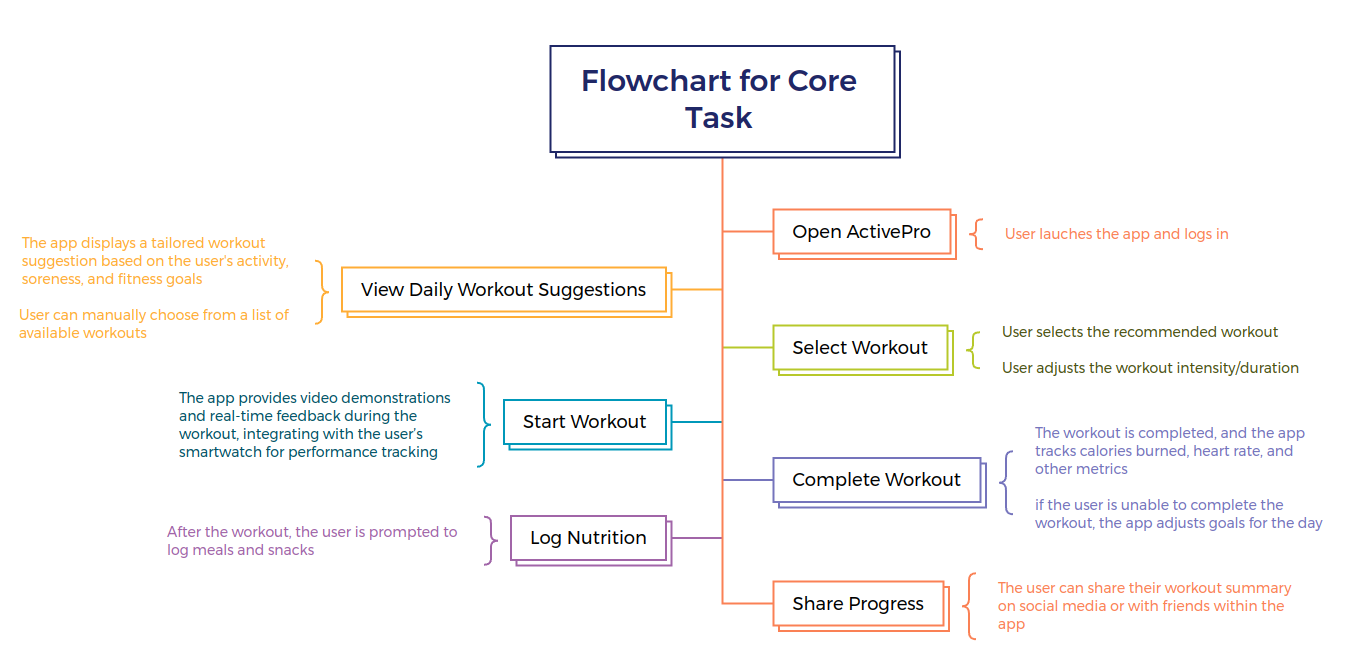
\includegraphics[width=18cm, height=12cm]{image5}
\end{figure}




%----------------------------------------------------------------------------------------

\end{document}